\chapter[In Memory of Prof.\ G Ramachandran: A tribute]{In Memory of\\ Prof.\ G Ramachandran:\\ A tribute}\label{chap5}

\Authorline{Prof.\ G. Bhamathi}

\begin{center}
University of Madras,\\
Chennai, India
\end{center}

I met Prof G Ramachandran as a fellow student when I joined the University of Madras for my Ph.D. degree, in 1959. I believe Prof.\ G. Ramachandran was two years my senior as Prof.\ Alladi Ramakrishnan's student.  There were about 10 or 12 of us registered for a Ph.D. degree under Prof.\ Alladi Ramakrishnan in various stages of progress. 

It was an unusual time and situation  to say the least. Prof.\ Ramakrishnan had been promoted to a professorship the previous year at the University Extension Centre at Madurai. How ever he preferred to commute between Madras and Madurai as there were not adequate library facilities for conducting research in Theoretical Particle Physics. Thus all his research students continued to stay in Madras and were asked to go to Madurai from time to time to assist in giving lectures on modern topics in Physics like mathematical physics, quantum mechanics, nuclear physics etc to the masters degree students of the affiliated colleges in Madurai.

For the research students in the Theoretical physics division in Madras there were no offices or class rooms where they could conduct their research or hold lectures and discussions. Instead lectures and discussions were held at the residence of Prof.\ Ramakrishnan, whenever he was in town. As far as doing research was concerned, students essentially worked at their own homes or in the libraries and met together when lectures were organized at Prof.\  Ramakrishnan's house. There were no fixed schedules for lectures nor any prescribed courses for entry level students. By and large there were one or two lectures daily  most of the week days. The lectures were  given mostly by the students themselves either on topics they were doing research on, or on topics assigned to them by Prof.\ Ramakrishnan. In addition to their own research, all the students were given the opportunity to assist Prof.\ Ramakrishnan in writing a book on Elementary Particle Physics, by being assigned different topics which formed the contents of the book.

Some of the lectures in Nuclear physics were given by Prof.\ G. Ramachandran. He was a very good teacher. He was meticulous in preparing the lectures and also provided lecture notes. 

During the three years of my Ph.D. days, several notable Physicists both from within India and from abroad who were already visiting other Indian Universities, were invited  by Prof.\ Ramakrishnan as guest lecturers. However since the University did not provide any funds for their support an informal association comprising all the students, called the Theoretical Physics Seminar, was created. Most of the guest lecturers were hosted by Prof.\ Ramakrishnan in his house and the funds collected by the Theoretical Physics Seminar, through a monthly contribution of the members,  were used to defray other expenses involved in the visit.

We were very fortunate that during those few years many scientists of international repute and leaders in their field like Niels Bohr, George Gamow, S. Chandrasekhar, Abdus Salam, Murray Gell-Mann, Richard Dalitz, Manoj Banerjee, Donald Glaser, E C G Sudarshan and several others visited the group. All the research students had  the opportunity to write notes for the lectures given by one or the other of the Visiting Professors.The lectures by these visitors provided a solid basis for all the students in their research pursuit. 

Prof.\ Alladi Ramakrishnan, left the University of Madras in 1962 to become  the Director of the newly created Institute of Mathematical Sciences. While most of the research students transferred to the Institute of Mathematical Sciences a few of us remained attached to the University of Madras.

As I was one of those that remained attached to the University of  Madras, after this point in time I did not have any interaction with Prof.\ G. Ramachandran until much later by which time I had become a Professor at the Department of Theoretical Physics in the University of Madras. We (Dept of Theoretical Physics) were conducting Summer courses for College Teachers in Madras in Quantum Mechanics, Nuclear Physics and a couple of other topics at an Advanced level so that the teachers were enabled to handle the Masters degree level courses. I was very pleased to find that Prof.\ Ramachandran retained the same passion for doing research in physics and teaching and spreading his knowledge to others as always. He retained his meticulous and methodical ways of instruction. The only difference I noted was that he had become more strict in observing his personal habits and ]insisted on cooking his own food daily. This observance and the fact that he stayed at a place quite far from the University campus meant that he had to work doubly hard during this period. 

He was an expert in the theory of angular momentum and had worked on pion production processes in low energy nuclear processes with Prof.\ V. Devanathan during the Ph.D. days. 

I believe an excellent teacher and a human being with a deep sense of commitment and integrity has been lost to the Indian scientific community with the passing of Prof.\ G. Ramachandran. I feel privileged to contribute to this memorial volume in honor of Prof.\ G. Ramachandran.

\vspace{1cm}

\centerline{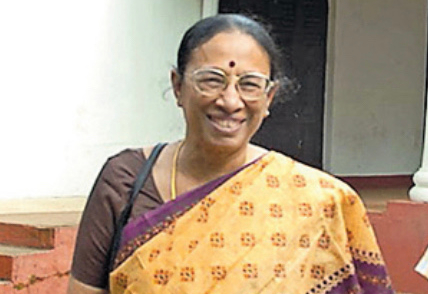
\includegraphics[scale=.4]{authorsphotos/G_Bhamathi.jpg}}
\smallskip

\authbio{G. Bhamathi}
\bigskip

\noindent
\textbf{Dr.\ Bhamathi} was a founder member of the Theoretical Physics Seminar Group which eventually became the Institute of Mathematical Science, Chennai. After obtaining her Ph.D. from the University of Madras under the guidance of Prof.\ Alladi Ramakrishnan, she joined the Physics Department, University of Madras. She retired as professor from Madras University in 1998. Currently she lives in Austin, Texas, USA.
